%% LyX 2.0.4 created this file.  For more info, see http://www.lyx.org/.
%% Do not edit unless you really know what you are doing.
\documentclass[12pt,ngerman,english,pointlessnumbers, abstracton, headsepline]{report}
\usepackage[T1]{fontenc}
\usepackage[latin9]{inputenc}
\usepackage{geometry}
\geometry{verbose,tmargin=2.5cm,bmargin=2.5cm,lmargin=2.5cm,rmargin=2.5cm}
\setcounter{secnumdepth}{3}
\setcounter{tocdepth}{3}
\setlength{\parskip}{\medskipamount}
\setlength{\parindent}{0pt}
\usepackage{color}
\usepackage{calc}
\usepackage{amsmath}
\usepackage{amssymb}
\usepackage{graphicx}
\usepackage{caption}
\usepackage{subcaption}

\makeatletter
%%%%%%%%%%%%%%%%%%%%%%%%%%%%%% User specified LaTeX commands.
\renewcommand\[{\begin{equation}}
\renewcommand\]{\end{equation}}

% for different coloured margin notes
\let\oldmarginpar\marginpar
\renewcommand\marginpar[1]
{\-\oldmarginpar[\color{red}\sffamily\raggedleft\scriptsize #1]%
{\color{red}\sffamily\raggedright\scriptsize #1}}



\usepackage{sverb}

\usepackage{geometry}

\geometry{verbose,a4paper}

% verschieden Symbole, Zeichen wie (c), �
\usepackage{textcomp}

%\addtokomafont{caption}{\footnotesize}
\usepackage [font=sf, size=footnotesize, labelfont={sf,bf}]{caption}

\usepackage{pdflscape}

\usepackage{ %a4wide,
            ellipsis, fixltx2e, mparhack,   %Fehlerkorrektur f�r Marginalien
            booktabs, longtable             %sch�nere Tabellen
}  

\usepackage[automark]{scrpage2}
%\automark[chapter]{chapter}
\clearscrheadfoot
\ohead{\\\headmark}
%\ihead{\includegraphics[scale=0.25]{pics/logo_schwarz.pdf}}%\pagemark}
\ofoot[\pagemark]{\pagemark}


%Kurzfassung und Abstract (englisch) auf eine Seite
\renewenvironment{abstract}{
    \@beginparpenalty\@lowpenalty
      \begin{center}
        \normalfont\sectfont\nobreak\abstractname
        \@endparpenalty\@M
      \end{center}
}{
    \par
}



% sch�nerer Blocksatz!!
\usepackage{microtype}

\usepackage{ifpdf} % part of the hyperref bundle
\ifpdf % if pdflatex is used

%set fonts for nicer pdf view
 \IfFileExists{lmodern.sty}{\usepackage{lmodern}}
  {\usepackage[scaled=0.92]{helvet}
    \usepackage{mathptmx}
    \usepackage{courier} }
\fi

 % the pages of the TOC are numbered roman
 % and a pdf-bookmark for the TOC is added
 \pagenumbering{roman}
 \let\myTOC\tableofcontents
 \renewcommand\tableofcontents{
   %\pdfbookmark[1]{Contents}{}
   \myTOC
   \clearpage
   \pagenumbering{arabic}}

%Bezeichungen anpassen
%Babelpaket mu� zuvor geladen werden
%\usepackage[ngerman]{babel}
%\addto\captionsngerman{ 
%\renewcommand{\figurename}{Abb.}% 
%\renewcommand{\tablename}{Tab.}% 
%\renewcommand{\abstractname}{Kurzfassung}
%\renewcommand{\nomname}{Abk�rzungen}
%}

% Alle Querverweise und URLs als Link darstellen
% In der PDF-Ausgabe
 \usepackage[colorlinks=true, bookmarks, bookmarksnumbered, bookmarksopen, bookmarksopenlevel=1,
  linkcolor=black, citecolor=black, urlcolor=blue, filecolor=blue,
  pdfpagelayout=OneColumn, pdfnewwindow=true,
  pdfstartview=XYZ, plainpages=false, pdfpagelabels,
  pdfauthor={LyX Team}, pdftex,
  pdftitle={LyX's Figure, Table, Floats, Notes, and Boxes manual},
  pdfsubject={LyX-documentation about figures, tables, floats, notes, and boxes},
  pdfkeywords={LyX, Tables, Figures, Floats, Boxes, Notes}]{hyperref}

%mehr Platz zwischen �berschrift und Tabelle
\newcommand{\@ldtable}{}
\let\@ldtable\table
\renewcommand{\table}{ %
                 \setlength{\@tempdima}{\abovecaptionskip} %
                 \setlength{\abovecaptionskip}{\belowcaptionskip} %
                 \setlength{\belowcaptionskip}{\@tempdima} %
                 \@ldtable}

%Aradi-style Schriftart
%\usepackage{mathpazo}

% Schriftgr��e auf 13 stellen
%\usepackage{type1cm}
%\renewcommand\normalsize{%
%   \@setfontsize\normalsize{13pt}{14.5pt}%
%   \abovedisplayskip 12\p@ \@plus3\p@ \@minus7\p@
%   \abovedisplayshortskip \z@ \@plus3\p@
%   \belowdisplayshortskip 6.5\p@ \@plus3.5\p@ \@minus3\p@
%   \belowdisplayskip \abovedisplayskip
 %  \let\@listi\@listI}\normalsize  

\makeatother

\usepackage{babel}
\begin{document}

\title{OSTI Phase 1: A Cellular Automaton Model of Early Tumor Growth and
Invasion}


\subtitle{The Effects of Native Tissue Vascularity and Increased Anaerobic
Tumor Metabolism by A.A. Patel et al.}


\subtitle{\rule[0.5ex]{1\linewidth}{1pt}\\
{\Large Systems Biology DTC 2012}}


\author{Jackie Ang, Alexander Erlich, Robert Ross, Jonathan Brooks-Bartlett,\\ James Mbewu\\
license CC-BY-SA-3.0}


\date{January 2013\\
University of Oxford\\
\foreignlanguage{ngerman}{{\normalsize \vspace{0.5cm}
}}}

\maketitle
\tableofcontents{}


\chapter{Introduction}


\subsection*{by Jackie Ang}

Cancer is a major cause of death worldwide and is defined as unregulated
cell growth within a structure known as a tumour. Tumour growth can
be classified into distinct stages, which are hyperplasia, dysplasia,
in situ carcinoma and finally invasive cancer. As tumours are made
up of rapidly dividing cells, they require high amounts of oxygen
and glucose for survival and cell division. This rapidly overwhelms
the ability of normal blood vessels to provide these nutrients and
leads to angiogenesis within the tumours. Also,
as a consequence of hypoxia within the tumour, cells switch to using
anaerobic respiration and release lactic acid into the extracellular
environment. This causes a decrease in the pH in the environment within
and around the tumour and also leads to necrosis. While the initiation of this switch to anaerobic respiration is often said to be an adaptation to the hypoxic environment, some investigators have found that it occurs even with an adequate oxygen supply and is a phenotypic consequence \cite{grif}\cite{roz}\cite{yama}. 

The resulting decrease in the environmental pH has deleterious effects on normal tissue as they have a much higher pH threshold for viability compared to tumour cells. Also, the decreased pH stimulates the production of enzymes which degrade the extracellular matrix and causes the loosening of gap junctions between cells. The degradation of extracellular matrix then allows the invasion of tumour cells into the host tissue. A discrete mathematical model involving all of these parameters as well as diffusion is thus useful for studying the interaction of tumour cells with its surrounding tissue as well as for the investigation of the changes within the microenvironment around the developing tumour. 

Cellular automata has a long history of usage to model the growth
and development of tumours. In this investigation by A.A. Patel et
al, a hybrid cellular automaton was used to model an early stage of
tumour growth. The cellular automaton assumes tumour avascularity
and a random distribution of blood vessels in a tissue, which is true
for pre-angiogenic tumours. The model includes variables for glucose
and lactic acid concentration. It however, does not include a variable
for oxygen concentration as the author is focusing on the effects
of acidification of the microenvironment rather than hypoxia. It was
shown that anaerobic respiration in tumour cells persists even
in high levels of oxygen and tumour cell viability is independent
of oxygen levels \cite{Gull}. 

\chapter{Methods }


\subsection*{by Jackie Ang et al.}


\section{Setup of Cellular Automaton }

First, a two-dimensional cellular automaton was created to model this tumour
growth. This was made up of a $N$ by $M$ array of elements with
a value corresponding to the state of each point. This state describes
the occupation status of each point, with values corresponding to
active normal cell, quiescent normal cell, necrotic normal cell, active tumour cell,
quiescent tumour cell, necrotic tumor cell and blood vessel. Although both necrotic normal cells
and necrotic tumor cells are effectively vacant elements (as referred to by Patel et al, in \cite{patel})
we made the distinction in the model so we could measure the radius of gyration of the tumor cells
which required the use of all states of tumor cells including the necrotic state. Active cells are 
allowed to divide whereas quiescent cells are not.\\

Two other $N$ by $M$ arrays of elements with positional conservation to the
first array were also created to represent the glucose and lactic
acid concentrations of each individual automaton element. This differs
from the authors in that they created a matrix of state-vectors each
containing four components which correspond to the same variables,
but leads to similar results. 

In \cite{patel} the authors also mentioned one of the four above components as ghost
values used only on elements occupied by vessels to enforce gradient
boundary conditions at the four walls of the vessels. However, this
has been covered In our program by fixing the glucose and lactic acid
concentrations in elements occupied by vessels and not allowing them
to change during the process of running the cellular automaton. 

The cellular automaton was randomly populated with microvessels using a user defined microvessel
density $\phi_{v}$ where 
\[
\phi_{v}=\frac{N_{v}}{N^{2}}
\]
where $N_{v}$ is the number of vessel elements inside the automaton. 

The program situates the vessel elements randomly, subject to the
condition that any given tumour cell or normal cell element can only
border a maximum of one vessel element. This is because if a cell element
borders two or more vessels, the value of the glucose and lactic concentrations
would be too strongly affected by the multiple boundary conditions
imposed by the vessels. 

All other elements within the cellular automaton were then populated
with active normal cells. Following this, a disc shaped group of
active tumour cells with a user defined diameter is introduced in
the centre of the automaton grid, replacing any normal cells or vessels
previously there. 

The other two $N$ by $M$ arrays are then populated with starting
values for glucose and lactic acid concentrations. For glucose concentrations,
a glucose profile is generated based on the diffusion equations and
the position of the vessels before the insertion of any non-vessel
cells. The glucose concentration at vessels however, is kept constant
at $G_{s}=5.0mM$. The lactic acid concentration is initialised at
all elements at $H_{s}=3.98\cdot10^{-5}mM$. This lactic acid concentration
corresponds to a pH of 7.4 in the extracellular environment.\\


\section{Rules of Cellular Automaton}

There are several rules for this cellular automaton as described below 
\begin{enumerate}
\item Elements occupied by microvessels do not change in status, glucose
and lactic acid concentrations in the entire simulation. 
\item Normal cells and tumour cells cannot evolve into other forms of cells.
They can only change status from active to quiescent or vice versa.
They may also die and this results in a vacant element (represented in code as a necrotic normal cell or a necrotic tumor cell if they were previously a normal or tumor cell respectively). 
\item If the occupancy of an automaton element is with a normal cell or
tumour cell, after each updating of glucose and lactic acid concentrations
of elements, if the local glucose concentration is below $G_{N}^{D}$
or $G_{T}^{D}$, which were both defined to be 2.5mM, the cell dies
and the occupancy becomes a corresponding necrotic cell. 
\item If there is enough glucose, the local lactic acid concentration of
the individual elements is then checked. For normal cells, if the
local lactic acid concentration exceeds $H_{N}^{D}$, defined as $1.58\cdot10^{-4}mM$
(pH 6.8), it becomes necrotic. Otherwise if the concentration of lactic acid is
between $H_{N}^{Q}$, defined as $7.94X10-5mM$ (pH 7.1) and $H^D_N$,
the cell survives but becomes quiescent. For tumour cells, if the
local lactic acid concentration is above $H_{D}^{T}$, defined as
$1\cdot10^{-3}mM$ (pH 6.0), it dies. Otherwise if the concentration
of lactic acid is between $H_{T}^{Q}$, defined as $3.98\cdot10^{-4}$
(pH 6.4) and $H_{T}^{D}$, it survives but becomes quiescent.
For a normal cell, if the local lactic acid concentration exceeds $H_{N}^{Q}$ then the normal cell
will become active. Similarly for the tumor cell, if the local lactic acid concentration exceeds $H_{T}^{Q}$ then the normal cell
will become active. 
\item Any cells that are now in an active state will be allowed
to divide. This can only occur if there is a vacant element adjacent
to the cell and can only occur once per cell even if there is more
than one vacant element adjacent to the cell. If there is more than
one vacant neighbour, the neighbouring element with the highest glucose
concentration will receive the daughter cell. 
\end{enumerate}

\section{Running the Simulation}

While there is a large disparity in the timescales of cell division($10^{2}$
hours) and diffusion of glucose and lactic acid($1 - 10$ seconds), it has been attempted to reconcile this difference
by stating that the distributions of nutrients and by products
do not change after reaching a steady state quickly and changes in
cell status can be treated as perturbations on the chemical distributions.

The problem of all cells responding simultaneously
to changes in chemical distributions has also been addressed by advancing the automaton in
a series of sub-generations. A generation is defined as the time taken
for all the elements within the automaton to be updated. For the purpose
of the simulations, the user defines number of subgenerations and hence the random fraction of cells that get updated each subgeneration (denoted by $f$) is calculated accordingly.

Importantly, at the start of a subgeneration a death\textunderscore matrix is initialised.  This stores the composition of the state\textunderscore matrix, i.e. cell types in cellular automaton, at the start of each subgeneration.  

Within each sub generation, a random subset $1/f$ of non-vessel
automaton elements are selected for updating.  This is acheived by iterating through $1/f$ of a randomised $N$*$M$ vector consisting of a number corresponding to each cell. This randomised $N$*$M$ vector is reinitialised at the beginning of every generation. The update takes the following order: 
\begin{enumerate}
\item The entire glucose and lactic acid fields are updated according to the solution of the equilibrium boundary value
problems.  
\item The state of the selected subgeneration of cells is then updated as quiescient, necrotic or active depending on the surrounding (cell right, left, up and down) pH and glucose fields. 
\item Following this, the death\textunderscore matrix, a representation of the state\textunderscore matrix at the start of the subgeneration is used to decide whether active cells from the current subgeneration state\textunderscore matrix can divide into free space created in previous subgenerations. This scheme means cells that have died in the current subgeneration cannot be occupied in the same subgeneration.  At the end of the subgeneration the death matrix is updated to the current state\textunderscore matrix, i.e. with the subgeneration changes, meaning that active cells in the next subgeneration are able to divide into the vacant grid elements.  
\end{enumerate}

\section{The GUI}
The graphical user interface (GUI) was made to visualise the results and is intended to summarise the most useful and important information in the simulation (see figure \ref{GUI}). When the "cancerModelGUI" script is run the GUI appears on screen with a list of the parameters on the right hand side of the screen. The user can input the parameters into the relevant text box in the GUI and then click the "RUN" button to see the results. The left hand side of the GUI contains the subplots that show the visual data produced when the code is run. The top left subplot shows the resulting state matrix after each full generation. The subplot on the top right handside of the GUI shows the radius of gyration of the tumor against the number of full generations that the simulation has completed (the radius of gyration is explained in section \ref{ROG}). The subplots on the bottom left and bottom right show the glucose concentration and the pH on the grid respectively. These subplots are updated every subgeneration.
\begin{figure}[h!]
   \centering
    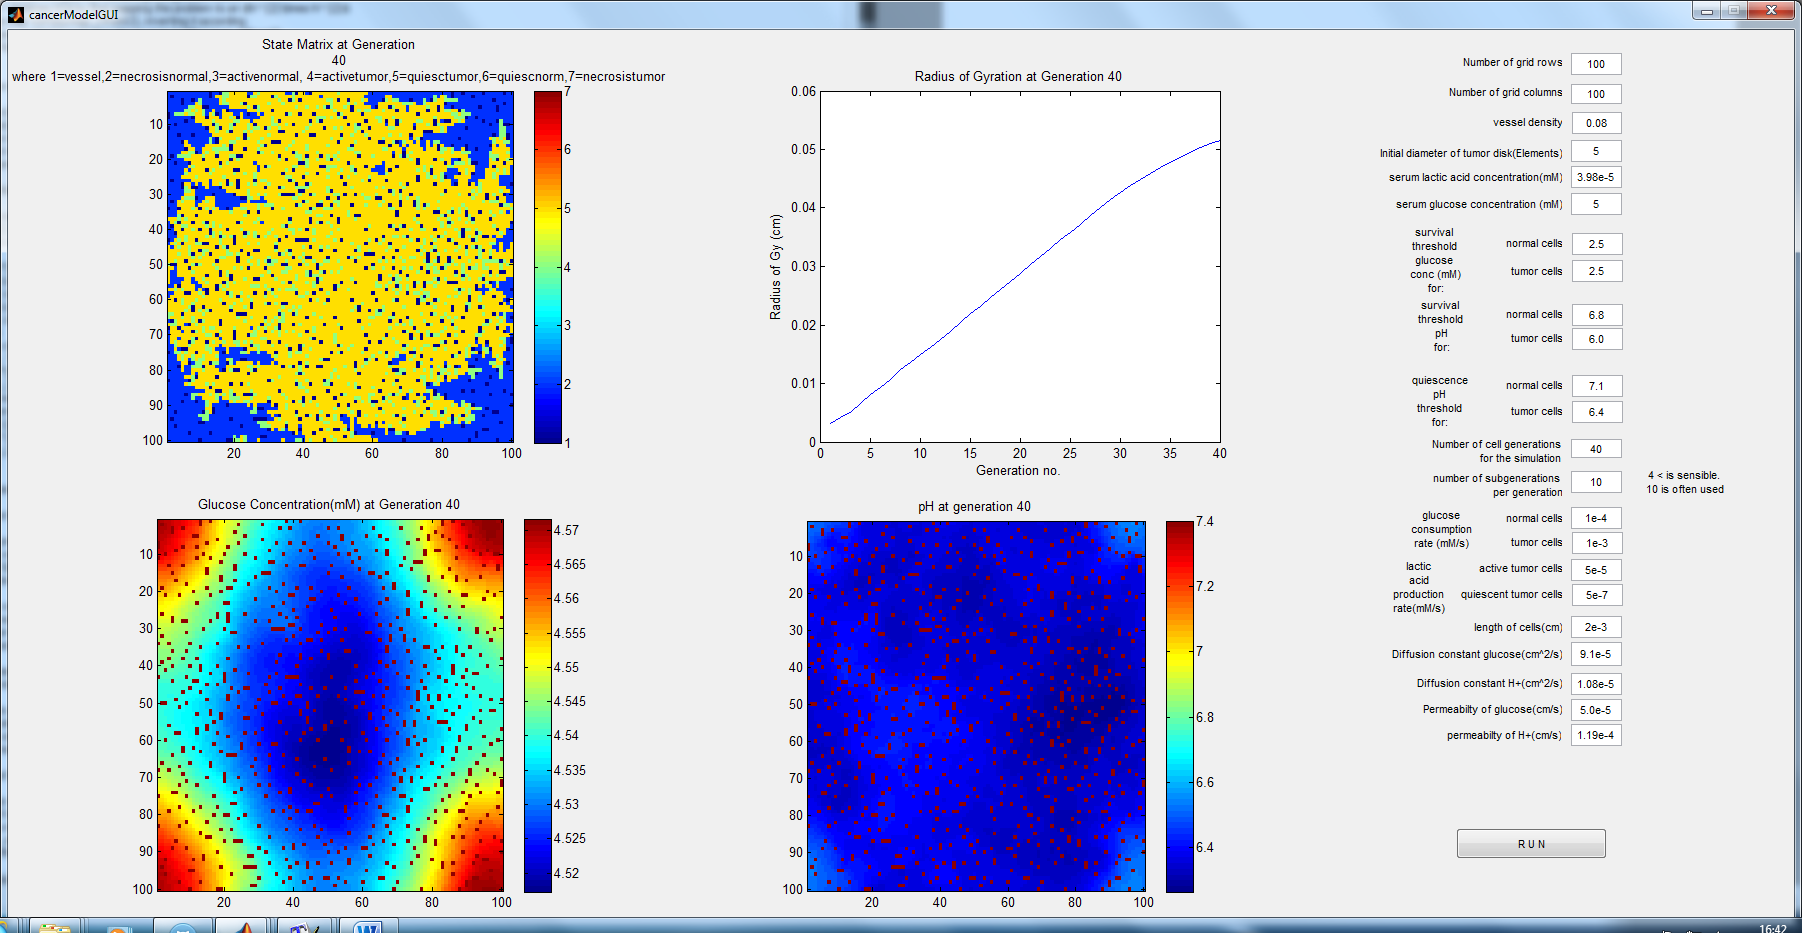
\includegraphics[width=1.0\textwidth]{GUI}
    \caption{Figure showing the GUI that has been created to display the results of the simulation}
    \label{GUI}
\end{figure}

\section{Glucose Inversion Problem}

The problem is to obtain a spatial solution of a steady state diffusion
equation
\begin{equation}
D_{G}\nabla^{2}G\left(\mathbf{r}\right)-k\left(\mathbf{r}\right)G\left(\mathbf{r}\right)=0\label{eq:diffusion_eqn}
\end{equation}
for the glucose concentration matrix $G$. The glucose consumption
rates are stored in the matrix $k$ as constants (we shall give further
information on this shortly). Here, $D_{G}$ is the glucose diffusion
constant (a scalar) and $G$, $K$ are an $N\times N$ matrices%
\footnote{It is slightly odd that the authors choose a lower case symbol for
a matrix but we shall stick to their notation. After all, $k\, G$
is a matrix product (summation over 2 indices). The authors might
have decided for this notation because$k$ is a matrix of constants,
i.e. $k=k\left(\mathbf{r}\right)$ but $k_{ij}\neq k_{ij}\left(\mathbf{r}\right)$. %
}. We want to solve this equation for the glucose concentration $G\left(\mathbf{r}\right)$,
i.e. on an $N\times N$ domain, with periodic boundary conditions. 

Let us define $G$ in $\mathbb{R}^{N\times N}$ , so in an orthonormal
basis $\left\{ \mathbf{e}_{k}\right\} $ we obtain 
\[
G=G_{i,j}\mathbf{e}_{i}\otimes\mathbf{e}_{j}
\]
which is a summation over indices $i,\, j$ (summation convention).
The periodic boundary condtions for the first index are
\begin{eqnarray*}
G_{0j} & \longrightarrow & G_{Nj}\\
G_{N+1,\, j} & \longrightarrow & G_{1,\, j}
\end{eqnarray*}
and the same for the other index. The cell distribution is expressed
through the matrix $k\left(\mathbf{r}\right)$ in terms of their glucose
consumption rates
\begin{equation}
k\left(\mathbf{r}\right)=\begin{cases}
k_{N} & \forall\mathbf{r}=\text{Normal Cells}\qquad1\cdot10^{-6}/s<k_{N}<5\cdot10^{-4}/s\\
k_{T} & \forall\mathbf{r}=\text{Tumor Cells}\qquad1\cdot10^{-5}/s<k_{T}<1\cdot10^{-3}/s\\
0 & \forall\mathbf{r}=\text{Vacant Cells}\qquad\text{no vacant cells at simulation startup}\\
0 & \forall\mathbf{r}=\text{Vessel Cells}
\end{cases}\label{eq:k_mat}
\end{equation}
The discretisation of \eqref{eq:diffusion_eqn} in terms of finite
differences can be written as
\begin{equation}
\frac{G_{i+1,j}+G_{i-1,j}+G_{i,j+1}+G_{i,j-1}-4G_{i,j}}{\Delta^{2}}-\frac{k_{i,j}G_{i,j}}{D_{G}}=0\label{eq:eqn_8}
\end{equation}
where the above mentioned diffusion constant is approximately $D_{G}\approx9.1\cdot10^{-5}cm^{2}/s$
and an automaton element is roughly of the size $\Delta^{2}\approx\left(20\mu\right)^{2}$
which is a rough approximation for cell size. At this point, we have
set up the system fully except for the vessel boundary conditions. 


\section{Vessel Boundary Conditions}

The reason why \ref{eq:eqn_8} unfortunately cannot be written as
a linear system $DG=K.*G$%
\footnote{meaning $\left(DG\right)_{ij}=D_{im}G_{mj}$ and $(K.*G)_{ij}=K_{ij}G_{ij}$,
not sure how to express that mathematically, I am just using Matlab
element wise notation. %
} is the vessel boundary conditions. If a vessel is placed at $i,\, j$
(corresponding to $k_{ij}=0$ since no vacant cells are allowed at
simulation startup, see \ref{eq:k_mat}) then $G_{ij}$ cannot be
accessed and therefore \ref{eq:eqn_8} must be modified.

If, for instance, a cell $\left(i,j\right)$ has a vessel to its right
($i,j-1$) then it cannot access this normal direction. Consequently,
we will treat this cell (at the boundary to a vessel to its left)
in terms of finite differences%
\footnote{There is an error in the paper, cf. eq. (13) on page 322.%
} as 
\begin{equation}
G_{i+1,j}+G_{i-1,j}+G_{i,j+1}-4G_{i,j}-\left(3+\frac{\Delta^{2}k_{i,j}+q_{G}\Delta}{D_{G}}\right)G_{i,j}=-\frac{q_{G}\Delta}{D_{G}}G_{S}\label{eq:eqn_13}
\end{equation}
where $G_{S}$ is the serum glucose value $G_{S}\approx5.0mM$ and
the permeability of the vessel wall is $q_{G}\approx3.0\cdot10^{-5}cm/s$.
Similarly, for a cell $\left(i,j\right)$ with a vessel at the above
/ below normal direction, the indices $\left(i-1,\, j\right)/\left(i+1,\, j\right)$
are not accessible and eqn. \ref{eq:eqn_13} must be adapted accordingly. 


\section{Numerical Approach}

We are interested in obtaining the elements of the glucose concentration
matrix 
\[
G\in\mathbb{R}^{N\times N}
\]
from the values of the glucose consumption rate matrix 
\begin{equation}
k\in\mathbb{R}^{N\times N}\label{eq:k_mat_general}
\end{equation}
 specified in \ref{eq:k_mat}. 

In order to be able to manipulate elements $G_{ij}$ individually,
we construct an $N^{2}\times N^{2}$ matrix $D$ and reformulate the
$N\times N$ matrix $G$ into a column vector $\mathbf{g}$ with $N^{2}$
elements. More precisely, if 
\[
G=\left(\mathbf{G}_{1}\quad\mathbf{G}_{2}\quad\cdots\quad\mathbf{G}_{N}\right)
\]
we choose
\[
\mathbf{g}=\begin{pmatrix}\mathbf{G}_{1}\\
\mathbf{G}_{2}\\
\vdots\\
\mathbf{G}_{N}
\end{pmatrix}\qquad\mathbf{g}\in\mathbb{R}^{N^{2}}
\]
and $D\in\mathbb{R}^{N^{2}\times N^{2}}$, $\mathbf{b}\in\mathbb{R}^{N^{2}}$,
$\mathbf{k}\in\mathbb{R}^{N^{2}}$ where the latter two are yet to
be constructed. As a result, we can formulate a linear matrix inversion
problem 
\begin{equation}
D\mathbf{g}=\mathbf{b}\qquad\mathbf{g}=D^{-1}\mathbf{b}\label{eq:inversion_problem}
\end{equation}
which will be a solution to \ref{eq:eqn_8} coupled to \ref{eq:eqn_13}.
In components, the problem reads
\[
\underbrace{\begin{pmatrix}D_{11} & \cdots & D_{N^{2}1}\\
\\
\\
\vdots &  & \vdots\\
\\
\\
D_{N^{2}1} & \cdots & D_{N^{2}N^{2}}
\end{pmatrix}}_{N^{2}\times N^{2}}\begin{pmatrix}G_{11}\\
\vdots\\
G_{N1}\\
G_{12}\\
\vdots\\
G_{NN}
\end{pmatrix}=\begin{pmatrix}\mathbf{G}_{1}\\
\mathbf{G}_{2}\\
\\
\vdots\\
\\
\mathbf{G}_{N}
\end{pmatrix}
\]
A map 1-to-1 map between $G\in\mathbb{R}^{N\times N}$ and $\mathbf{g}\in\mathbb{R}^{N^{2}}$
can be worked out. If $i,\, j$ are the indices of $G$ and $c$ is
the element number of $\mathbf{g}$, we get routines

\begin{eqnarray}
{\tt function\,\, C} & {\tt =} & {\tt CfromIJ(I,\, J,\, N)}\label{eq:map_CfromIJ}\\
{\tt function[I,\, J]} & {\tt =} & {\tt IJfromC(C,\, N)}\label{eq:map_IJfromC}
\end{eqnarray}
\textbf{In simple terms}, the goal is in obtaining the glucose matrix
$G\in\mathbb{R}^{N\times N}$ by first mapping the problem to an $N^{2}\times N^{2}$
problem using the map \ref{eq:map_CfromIJ}, inverting it according
to \ref{eq:inversion_problem} and using the inverse \ref{eq:map_IJfromC}
to obtain values for $G$. 


\section{Inversion Algorithm for the Glucose Matrix}

\framebox{\begin{minipage}[t]{1\columnwidth}%
\begin{enumerate}
\item Identify the indices $i^{*},\, j^{*}$ in $k_{ij}$ (see eq. \ref{eq:k_mat_general})
on which a vessel is placed. Use the map \ref{eq:map_CfromIJ} to
obtain $c^{*}$ and set
\[
D_{c^{*}k}=\delta_{c^{*}k}\quad\Leftrightarrow\quad G_{i^{*}j^{*}}=1
\]
i.e. update one row in D.
\item Consider the four neighbors in the normal directions corresponding
to indicies
\begin{eqnarray*}
i^{*}-1,\, j^{*} &  & \text{cell above vessel}\\
i^{*}+1,\, j^{*} &  & \text{cell below vessel}\\
i^{*},\, j^{*}-1 &  & \text{cell to the left of vessel}\\
i^{*},\, j^{*}+1 &  & \text{cell to the right of vessel}
\end{eqnarray*}
and update them taking account of the boundary conditions, i.e. by
\ref{eq:eqn_13}. This corresponds to updating rows in $D$. Also
update $b_{c^{*}}=-q_{G}\Delta G_{S}/D_{G}$. Use \ref{eq:map_CfromIJ}
and \ref{eq:map_IJfromC} to switch between the representations.
\item Update all remaining cells according to \ref{eq:eqn_8}, switching
between representations by \ref{eq:map_CfromIJ} and \ref{eq:map_IJfromC}.
\item Find $D^{-1}\in\mathbb{R}^{N^{2}\times N^{2}}$ by eqn. \ref{eq:inversion_problem}
and reshape $D^{-1}$ into $G\in\mathbb{R}^{N\times N}$, \ref{eq:map_CfromIJ}
and \ref{eq:map_IJfromC} to convert.\end{enumerate}
%
\end{minipage}}


\section{Acid Profile}

Even though the acid profile is just as important as the glucose concentration
for the cellular automaton algorithm we shall treat it very briefly
in this section because it is analogous to the glucose profile. To
obtain the acid profile, we need to solve Poisson's equation
\begin{equation}
D_{H}\nabla^{2}H\left(\mathbf{r}\right)+h\left(\mathbf{r}\right)=0\label{eq:Lactic_Acid_Eqns}
\end{equation}
where the lactic acid diffusion constant is $D_{H}\approx1.08\cdot10^{-5}\text{cm}^{2}/s$
and $H\left(\mathbf{r}\right)$ is the $\text{H}^{+}$ concentration.
Similarly to $k\left(\mathbf{r}\right)$ in eqn. \ref{eq:k_mat},
$h\left(\mathbf{r}\right)$ is a matrix of constants $h=h\left(\mathbf{r}\right)$
but $h_{ij}\neq h_{ij}\left(\mathbf{r}\right)$. It is defined as
\begin{equation}
h\left(\mathbf{r}\right)=\begin{cases}
\dot{H}_{T}^{A} & \forall\mathbf{r}=\text{Active tumor cells}\qquad1\cdot10^{-5}\,\text{mM/s}<\dot{H}_{T}^{A}<1\cdot10^{-4}\,\text{mM/s}\\
\dot{H}_{T}^{Q} & \forall\mathbf{r}=\text{Quiescent tumor cells}\qquad\dot{H}_{T}^{Q}=5\cdot10^{-7}\,\text{mM/s}\\
0 & \forall\mathbf{r}\neq\text{Tumor cells}
\end{cases}\label{eq:Lactic_Acid_Rates}
\end{equation}
where $\dot{H}_{T}^{A}$ and $\dot{H}_{T}^{Q}$ are the lactic acid
production rates for active and quiescent tumor cells. 

The solution of \ref{eq:Lactic_Acid_Eqns} with \ref{eq:Lactic_Acid_Rates}
can be obtained in absolute analogy to eqn. \ref{eq:eqn_8} and \ref{eq:eqn_13},
with these slight adaptations:
\begin{enumerate}
\item Replace $D_{G}\rightarrow D_{H}$, $q_{G}\rightarrow q_{H}$, $G_{S}\rightarrow H_{S}$
where the lacitic acid diffusion constant $D_{H}$ has been introduced
previously, the vessel permeability to lacitic acid is $q_{H}\approx1.19\cdot10^{-4}\,\text{cm/s}$
and the serum acid concentration ($\text{pH}=7.4$) is $H_{S}=3.98\cdot10^{-5}\text{\, mM}$.
\item Replace $k_{i,j}G_{i,j}\rightarrow k_{i,j}$ because we are considering
Poisson's equation now. 
\end{enumerate}
With these considerations, the algorithm described above for glucose
applies to the lactic acid as well. 
\section{Calculating Tumour Size and Growth Rate}
\label{ROG}

To analyse the model tumour size was characterised by its radius of gyration as 
was done by Patel \emph{et al.} \cite{patel}. The tumour size was calculated 
including regions of active and quiescent tumour cells as well as tumour necrosis 
(i.e. where tumour cells have died). The radius of gyration $R_G$ can be calculated 
as the square root of the second moment of the spatial distribution ($J$) 
divided by the total area of the spatial distribution ($A$), i.e.

\begin{equation}
R_G = \sqrt{\frac {J} {A} },
\end{equation}

returning a measure of the radius of the tumour (in this text reported in \emph{cm}). 
The second moment of the spatial distribution can be calculated using the following 
formula:

\begin{equation}
J = \sum^{no. cells} {J_{cell} + y^2 A_{cell}}.
\end{equation}

where $J_{cell} = \frac{l^4}{12}$ is the second moment of area of an individual 
square cell ($l=20\mu m$ is the length of each cell), $y$ is the distance in the 
$y$-direction to the centroid of the tumour and $A_cell = l^2$ is the area of each 
individual cell.

Note that in the original paper by Patel et al., the radius of gyration was stated 
as being square root of the second moment of area. However, this was clearly a 
mistake and their results corresponded to the above definition of the radius of 
gyration.

To analyse the growth rate of each tumour in each simulation, the radius of gyration 
for the last ten generations (out of a total of 40 generations) was analysed 
using linear regression to find the slope (i.e. tumour growth rate) of the regression 
line. This was generally an accurate representation of the growth rate since 
after an initial transient period, tumour size increased linearly (see Figure 
\ref{tg}).

\chapter{Results}
Figure \ref{tg} shows tumour size, as given by radius of gyration, with respect to generation number.  Prior simulations allowed it to be gauged that tumour growth would only occur in the model above a lactic acid production of $4.75\times10^{-5}mM$.  As can be seen, increasing acidity decreases growth rates in agreement with the Patel et.al paper (2001). This is because high lactic acid concentration kills normal cells while cancer cells have a higher resistance, and so therefore cancer cells are fitter in a more acidic environment.\\
Figure \ref{grap} shows growth rate vs. acid production, with the five plotted lines corresponding to different vessel distributions as given in the legend.  It can be seen that increased vessel density increases growth rate generally, although not at all time points.  In contrast, increasing acid production seems to affect growth rate but not in an easily understandable way.  Figure \ref{grvd} shows growth rate vs. vessel fraction, with the five plotted lines corresponding to different tumour acid production.  It can be seen that as in figure \ref{grap} increasing vessel density increase growth rate regardless of lactic acid production rate.  However, it appears that beyond a vessel density of 0.2 it becomes an inhibiting factor.  In the \cite{patel} paper this in confirmed with growth rate decreasing with beyond a certain vessel density threshold.


\begin{figure}[h!]
   \centering
    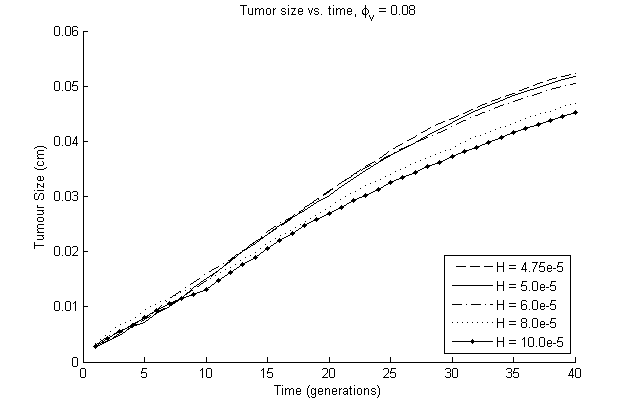
\includegraphics[width=0.5\textwidth]{tumourGrowth}
    \caption{Graph showing the tumour size against the number of generations in the simulation}
    \label{tg}
\end{figure}

\begin{figure}
        \centering
        \begin{subfigure}[t]{0.5\textwidth}
                \centering
                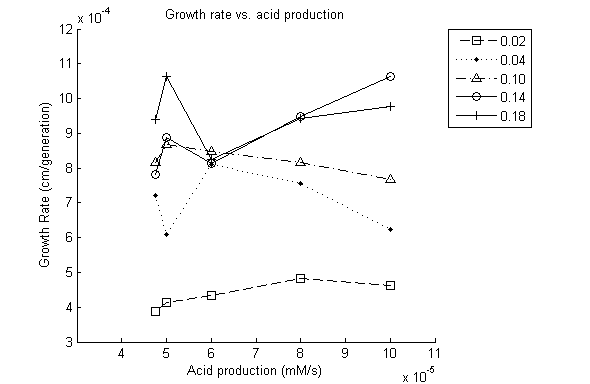
\includegraphics[width=\textwidth]{Growth_rateAcid_Production}
                \caption{}
                \label{grap}
        \end{subfigure}%
        \begin{subfigure}[t]{0.5\textwidth}
                \centering
                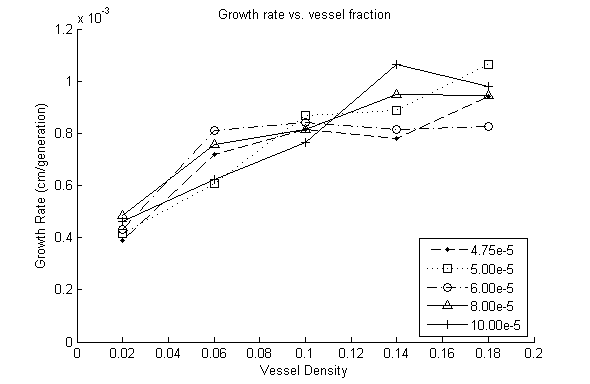
\includegraphics[width=\textwidth]{Growth_rateVessel_Density}
                \caption{}
                \label{grvd}
        \end{subfigure}
        \caption{Figure (a) shows a graph showing the growth rate of the tumour vs the lactic acid production of the tumour cells. The results were plotted using different values for the vessel density in each simulation given in the legend. Figure (b) shows a graph showing the growth rate of the tumour vs the vessel density. The results were plotted using different values for the lactic acid production for the tumour cells in each simulation given in the legend.}\label{grav}
\end{figure}

As can be seen from Figure \ref{many} the glucose concentration 
does not vary a great deal in magnitude. In fact, the glucose level at 
which cell death occurs of $2.5mM$ ($G_D$ and $G_T$) in the cellular automaton 
rules was never reached in our simulation. This is in correspondence with results 
of \cite{patel} and indicates that cells never die because of 
lack glucose, but only because of acidosis (high acid concentration). The 
glucose concentration does affect the simulation however, by controlling the 
direction in which cells divide in the automaton rules. This may be the cause 
of distinct cross shaped tumours for selected parameters.

Another feature of tumour growth is that the tumour inhibits its own growth 
by creating a high pH in and around itself. This can be seen in Figure \ref{many} 
where the interior of the tumour is quiescent (coloured yellow) while 
at the outside of the tumour the cells are active and dividing (coloured green). 
Another thing to note is that in the interior, close to vessels (coloured blue), 
there are a number of active cells. This is because at these locations the pH 
is increased due to the proximity to the vessels which have a high pH and do not 
inactivate the tumour cells.

Also noticeable in the plots of cell state is the ring of dead cells in which tumour 
cells divide as well as a ring of quiescent normal cells. The ring of dead cells, 
termed the hypocellular gap, has been reproduced as predicted by Gatenby \emph{et al.} 
\cite{gate} as well as in the paper this work was based on.

\begin{figure}
        \centering
        \begin{subfigure}[t]{0.25\textwidth}
                \centering
                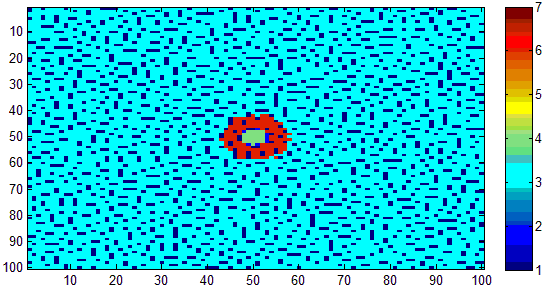
\includegraphics[width=\textwidth]{cellStateGen1}
                
                \label{}
        \end{subfigure}\qquad
        \begin{subfigure}[t]{0.25\textwidth}
                \centering
                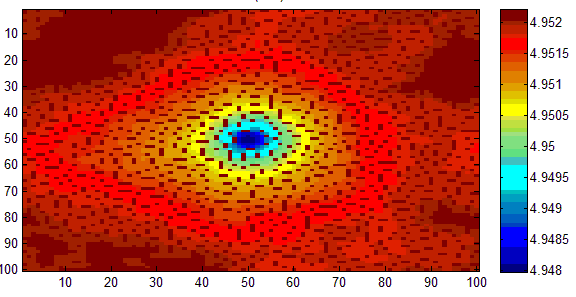
\includegraphics[width=\textwidth]{glucoseGen1}
                
                \label{}
        \end{subfigure}\qquad
        \centering
        \begin{subfigure}[t]{0.25\textwidth}
                \centering
                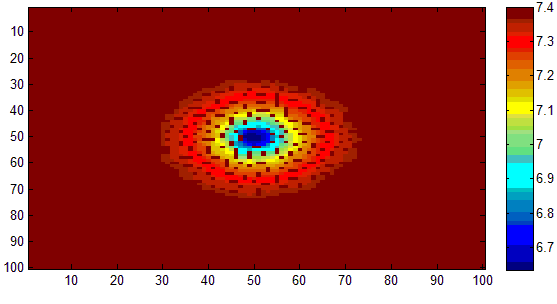
\includegraphics[width=\textwidth]{pHGen1}
                
                \label{}
        \end{subfigure}\\
        \centering
        \begin{subfigure}[t]{0.25\textwidth}
                \centering
                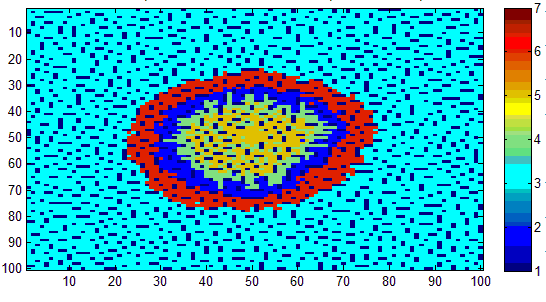
\includegraphics[width=\textwidth]{cellStateGen11}
                
                \label{}
        \end{subfigure}
        \begin{subfigure}[t]{0.25\textwidth}
                \centering
                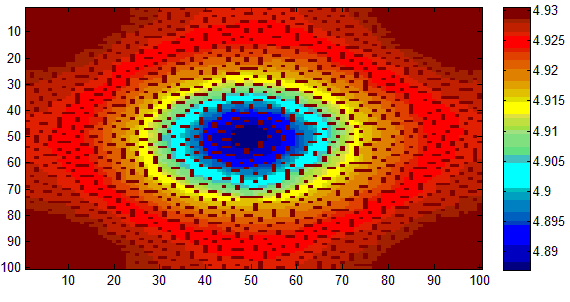
\includegraphics[width=\textwidth]{glucoseGen11}
                
                \label{}
        \end{subfigure}\qquad
        \centering
        \begin{subfigure}[t]{0.25\textwidth}
                \centering
                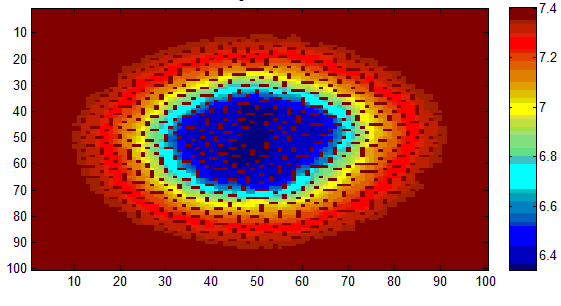
\includegraphics[width=\textwidth]{pHGen11}
                
                \label{}
        \end{subfigure}\\
        \centering
        \begin{subfigure}[t]{0.25\textwidth}
                \centering
                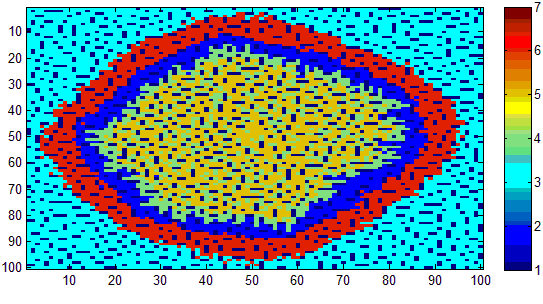
\includegraphics[width=\textwidth]{cellStateGen21}
                
                
        \end{subfigure}\qquad
                \centering
        \begin{subfigure}[t]{0.25\textwidth}
                \centering
                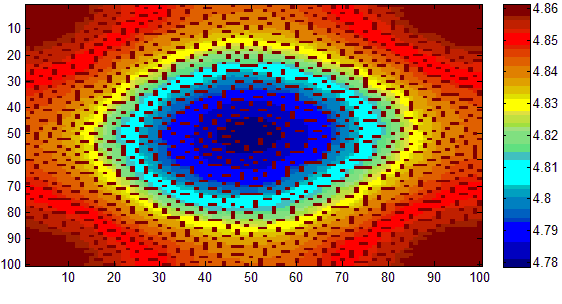
\includegraphics[width=\textwidth]{glucoseGen21}
                
                
        \end{subfigure}\qquad
        \begin{subfigure}[t]{0.25\textwidth}
                \centering
                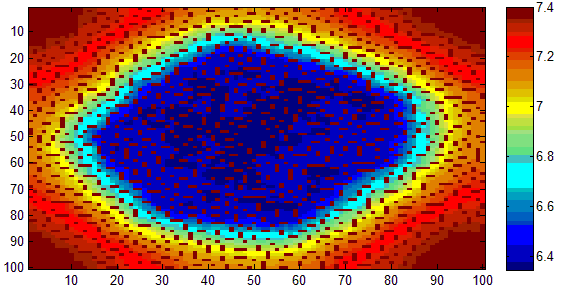
\includegraphics[width=\textwidth]{pHGen21}
                
                
        \end{subfigure}\\
        \centering
                \begin{subfigure}[t]{0.25\textwidth}
                \centering
                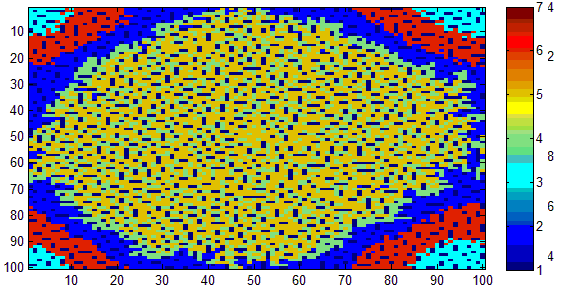
\includegraphics[width=\textwidth]{cellStateGen31}
                
                
        \end{subfigure}\qquad
                \centering
        \begin{subfigure}[t]{0.25\textwidth}
                \centering
                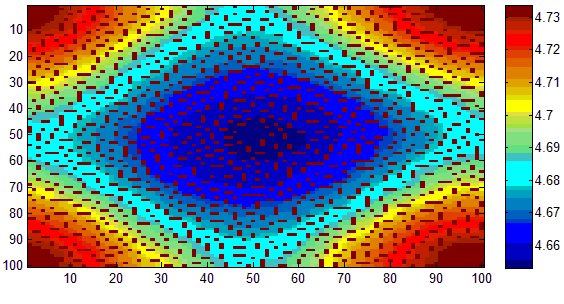
\includegraphics[width=\textwidth]{glucoseGen31}
                
                
        \end{subfigure}\qquad
        \begin{subfigure}[t]{0.25\textwidth}
                \centering
                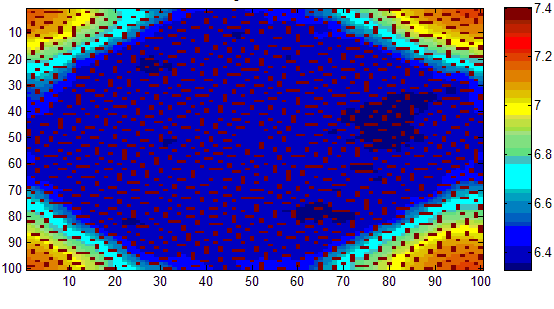
\includegraphics[width=\textwidth]{pHGen31}
                \end{subfigure}\\
        
              
        
        \caption{The temporal evolution of a tumour using the model described in this text (with 
parameters $\phi_v = 0.18$, and $H_{T}^{A} = 4.75\times 10^-5 mM/s$) with 
100$\times$100 automaton elements. In the first column the cell state is shown, 
with numbers corresponding to 1) vessel, 2) dead normal cell, 3) active normal 
cell, 4) active tumour cell, 5)  quiescent tumour cell, 6) quiescent tumour 
cell and 7) dead tumour cell. The tumour is plotted at generations 1, 11, 21 
and 31. The hypocellular ring is clearing visible infront of the advancing tumour.}\label{many}\end{figure}
        
\chapter{Discussion}

\section{Problems Faced with Original Paper and Differences}

We faced a few problems in the interpretation of the original paper by Patel et al. \cite{patel}. The first issue is with regards to the pH and lactic acid conversion. The author uses lactic acid concentration as well as pH at various points within the original paper without linking the two. There is no conversion scale between the two except for a mention that a lactic acid concentration of $3.98\cdot10^{-5}mM$ corresponds to a pH of 7.4. We had to make a few physiologically incorrect assumptions in order to make the model work. These were to assume lactic acid secretion by tumour cells was the only source of hydrogen ions, the hydrogen ions released were not neutralised or buffered and the pKa of lactic acid was constant. 

Another problem we faced was with the order of updating the cellular automaton. The author stated that cellular element states were updated after the chemical fields were updated. However, there was no order as to which status changes were updated first and no mention as to whether quiescent cells can turn active. For our simulations, we have assumed that quiescent cells can turn active if the pH is above the threshold for quiescence. It was also not clear from the paper whether cells could divide into the 4 adjacent spaces only or into all 8 neighbouring spaces. In this cellular automata, we have made the choice of division into 4 possible spaces only. 

As a result of these problems with the interpretation of the paper, it is very possible that our cellular automata differs considerably from the original by Patel et al. \cite{patel}. It is possible, in addition to the problems mentioned above, that different pde solvers were used and this would affect the values of both the chemical fields, leading to the differences in the results seen.

The results of this cellular automata are significantly different from that of the original by Patel et al. \cite{patel} For instance, the tumour did not grow in our simulations unless the tumour acid production rate was at least  $4.75\cdot10^{-5}mM/s$ while it grew even with an acid production rate of  $2.5\cdot10^{-5}mM/s$ in the original paper. While the trends seen are similar, more differences are also evident in (Figures \ref{grap} and \ref{grvd}). In Figure \ref{grvd}, the growth rate does not decrease even with a vessel density of 0.20, which is unlike the original where the growth rate decreases when the vessel density is 0.18 or above. 

\section{Biological Significance and Future Work}

Our hybrid cellular automaton explores the effects of vessel density and tumour acid production on the growth and development of avascular, early stage tumours. While this is not completely representative of all tumours, it is still a useful model for this purpose as it is able to capture many of the known characteristics of tumour growth and compares well with real life tumours. Our model also allows many parameters to be user defined and this allows any user to adjust any combination of many parameters which include survival and quiescence thresholds of both normal and tumour cells, starting glucose and lactic acid concentrations as well as the size of the initial tumour. This is an improvement on the original automaton and would be useful for investigations where are are different values of these parameters, among others. 

Future work on our cellular automaton should include the expansion of this automaton to include parameters for oxygen as well as its diffusion as hypoxia is also an important factor for tumour growth. An angiogenesis simulation can also be included in order to expand the simulation past the avascular growth stage. However, both of these improvements would require further research on the values of parameters required as well as the development of a completely new angiogenesis function. 


\bibliography{References}
\bibliographystyle{plain}

\end{document}
